\chapter{Wartungsansätze und Framework}\label{ch:pdm_theorie}
\section{Wartungsansätze}
Die zunehmende Komplexität und Vernetzung moderner Systeme erfordert effizientere Wartungsstrategien. Predictive Maintenance nutzt die
enormen Datenmengen solcher Systeme, um drohende Defekte frühzeitig zu erkennen und Ausfälle zu verhindern. Dadurch können
Ausfallzeiten minimiert und die Lebensdauer der Systeme verlängert werden.

Im Vergleich zu traditionellen Ansätzen bietet Predictive Maintenance signifikante Vorteile,
doch auch die klassischen Methoden haben ihre Berechtigungen. Diese werden im Folgenden diskutiert.

\subsection{Traditionelle Wartungsansätze}\label{sec:trad_maintenance}
Zu den traditionellen Wartungsansätzen gehören die reaktive und die präventive Wartung. Bei der reaktiven oder auch korrektiven
Wartung wird, gemäß der Namensgebung, erst bei vollständigem Ausfall von Komponenten gehandelt.
Der Vorteil dieser Methode liegt in der sehr geringen Planung und Überwachung. Für Komponenten,
die nicht kritisch oder essenziell sind, oder die ein sehr geringes Ausfallrisiko aufweisen, kann die reaktive Wartung sinnvoll sein.
Für alle anderen Bestandteile bzw.~die Gesamtheit eines Systems ist sie jedoch höchst ineffizient, da Wartungsmaßnahmen erst dann
veranlasst und geplant werden, wenn das System ausfällt. Zudem gestaltet sich die Diagnose dann auch als potenziell schwierig, da die
Fehlerquelle noch gefunden werden muss~\cite{Abdelli2022}.

Demgegenüber steht die präventive Wartung, die Maßnahmen am Ende eines vorher festgelegten Zeitintervalls oder nach Ablauf einer
bestimmten Betriebsdauer festlegt. Diese Zeitintervalle werden beispielsweise anhand der Badewannenkurve~\cite[S.~4]{Andrews2002},
wie in \hyperref[fig:bathtub]{Abb.~\Ref*{fig:bathtub}} dargestellt, auf Basis von Erfahrungswerten oder empirischen Untersuchungen geschätzt.
Die Badewannenkurve ist eine Darstellung der Ausfallverteilung, die die Wahrscheinlichkeitsverteilung von mechanischen oder elektrischen
Defekten beschreibt. Dieser Ansatz hat gewisse Vorteile für Komponenten, die nicht im dauerhaften Betrieb sind, sofern ausreichend geschultes Personal vorhanden
ist mit genügend Zeit, die Wartungsarbeiten durchzuführen. Nachteile liegen im potenziell schlechten Timing der Wartungsarbeiten, die
entweder zu früh oder zu spät stattfinden. Ohne Überwachung des Systemzustands ist schwer absehbar, in welchem Stadium seiner Lebensdauer
sich ein System befindet, und Komponenten, die noch eine gewisse Zeit weiterlaufen könnten, werden zu früh ausgetauscht. Durch die Wartung
verkürzt sich auch die Betriebsdauer des ganzen Systems und verursacht vermeidbare Kosten~\cite{Scheffer2004}.

\begin{figure}[H]
    \centering
    \begin{tikzpicture}
        \node[anchor=south west,inner sep=0] (image) at (0,0) {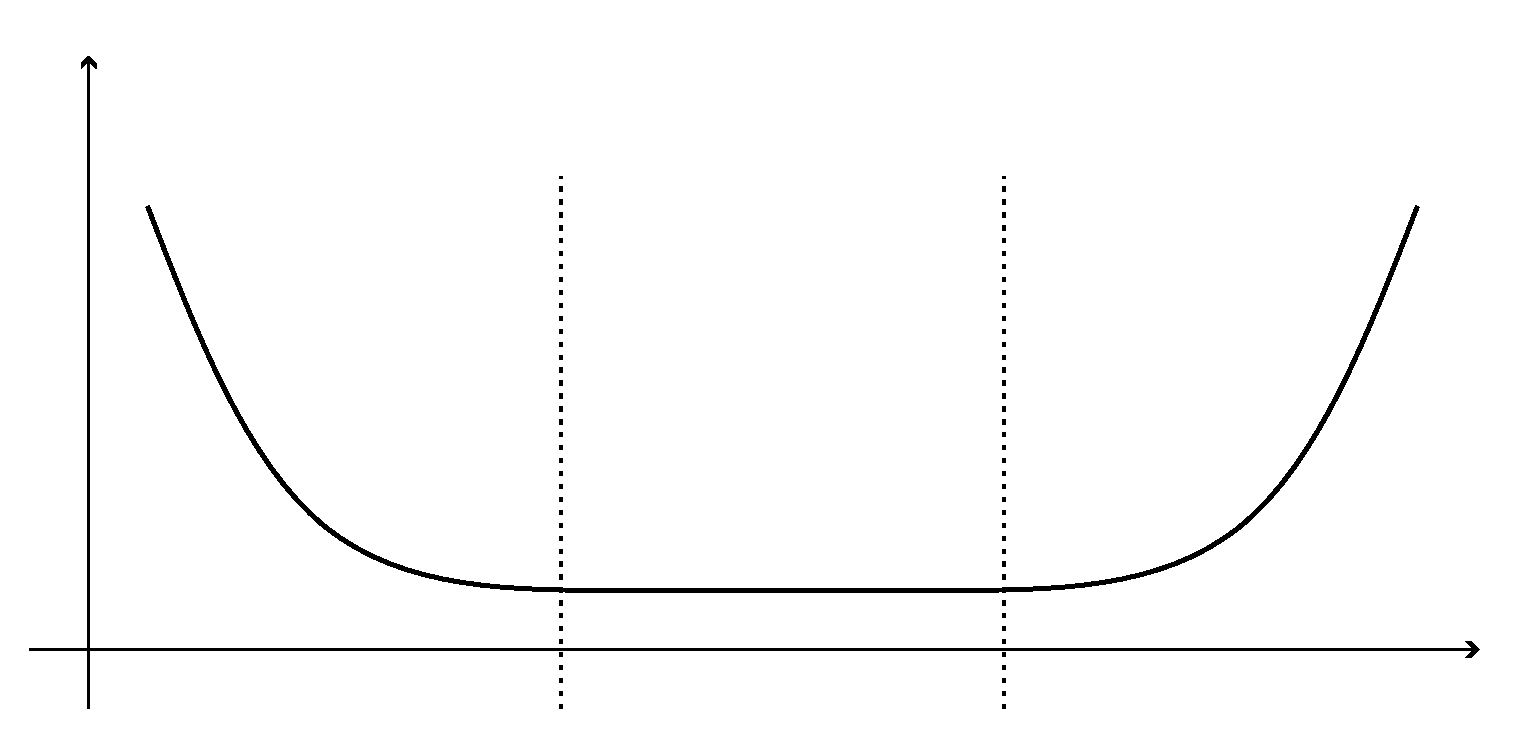
\includegraphics[width=\linewidth]{ch3_theorie_framework/abbildungen/bathtub.pdf}};
        % Koordinatensystem für die Grafik
        \begin{scope}[x={(image.south east)},y={(image.north west)}]
            % Textpositionen anpassen:
            \node at (0.25,0.92) {\large\parbox{6cm}{Ausfallwahrscheinlichkeit}};
            \node at (0.88,0.05) {\large\centering Betriebsdauer};
            \node at (0.25,0.6) {\large\parbox{4cm}{\centering I\\Frühausfälle}};
            \node at (0.51,0.6) {\large\parbox{6cm}{\centering II\\normale Lebensdauer}};
            \node at (0.77,0.6) {\large\parbox{4cm}{\centering III\\Alterserscheinungen}};
        \end{scope}
    \end{tikzpicture}
    \caption{Badewannenkurve zur Visualisierung der Ausfallverteilung}
~\label{fig:bathtub}
\end{figure}

\subsection{Predictive Maintenance}
Nach Mobley~\Cite[S.~4]{Mobley2002} wird Predictive Maintenance als eine zustandsbasierte Wartungsstrategie definiert, die den
tatsächlichen Betriebszustand von Anlagen und Systemen überwacht, um Wartungsaktivitäten bedarfsgerecht zu planen.
Eine passende Analogie findet sich in der Medizin: Wenn der menschliche Körper Anzeichen einer bevorstehenden Krankheit zeigt, können
diese Symptome vom Arzt genutzt werden, um eine Diagnose zu stellen. Dementsprechend werden dann Maßnahmen ergriffen, zum Beispiel
wird eine Behandlung eingeleitet oder Medikamente verordnet. Diese Zustandsüberwachung erlaubt es, dass Wartungsarbeiten zu einem
Zeitpunkt stattfinden können, der für alle Beteiligten passend ist und minimale Einschnitte in Produktions- oder Prozesslaufzeiten
bedeutet~\cite[S.~3]{Scheffer2004}.

Anhand von \hyperref[fig:pdm_workflow]{Abb.~\Ref*{fig:pdm_workflow}} ist zu erkennen, welche vereinfachten Schritte zur erfolgreichen
Implementierung eines Predictive Maintenance Systems erforderlich sind. Essentiell ist an erster Stelle eine adäquate Infrastruktur, die
sämtliche Zustandsparameter erfasst und gleichzeitig in der Lage ist, die erfassten Daten auch bereitzustellen. Es müssen im nächsten
Schritt Daten gesammelt werden, damit die im normalen Betriebszustand gültigen Schwellwerte ermittelt und festgelegt werden können.
Anhand dieser wird dann im laufenden, mittlerweile aufgenommenen Betrieb festgestellt, ob Abweichungen von den Parametern im Normalbetrieb
vorliegen. Demnach werden notwendige Wartungsarbeiten geplant und vorbereitet, wonach der Betrieb wieder ordnungsgemäß aufgenommen werden
kann.

\begin{figure}[H]
    \centering
    \begin{tikzpicture}
        \node[anchor=south west,inner sep=0] (image) at (0,0) {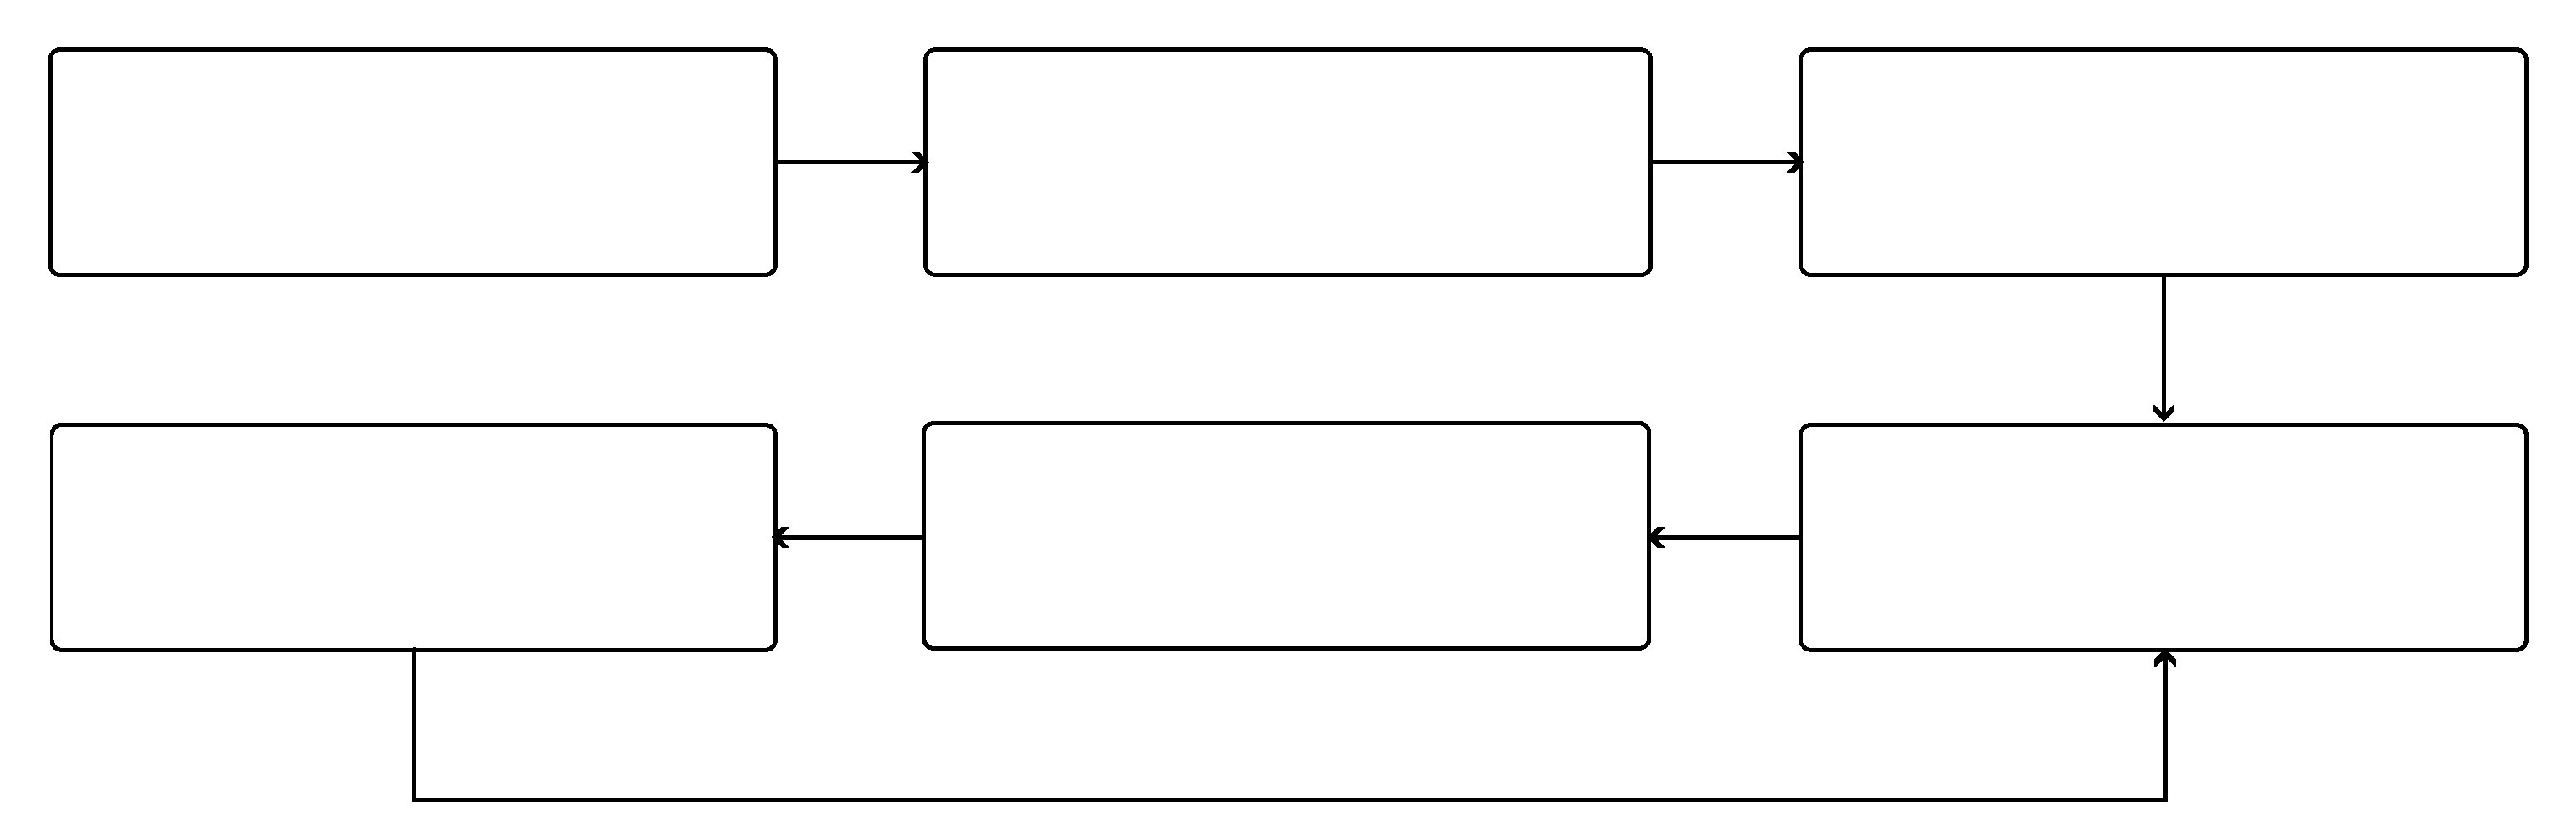
\includegraphics[width=\linewidth]{ch3_theorie_framework/abbildungen/pdm_workflow.pdf}};
        % Koordinatensystem für die Grafik
        \begin{scope}[x={(image.south east)},y={(image.north west)}]
            % Textpositionen anpassen:
            \node at (0.16,0.815) {\large\parbox{6cm}{\centering Zustandsüberwachung\\einrichten}};
            \node at (0.5,0.815) {\large\parbox{6cm}{\centering Daten aggregieren}};
            \node at (0.84,0.815) {\large\parbox{6cm}{\centering Schwellwerte festlegen \&\\Parameter setzen}};
            \node at (0.84,0.35) {\large\parbox{6cm}{\centering normale\\Betriebsaufnahme}};
            \node at (0.5,0.35) {\large\parbox{6cm}{\centering Anomalien im\\Betrieb feststellen}};
            \node at (0.16,0.35) {\large\parbox{6cm}{\centering Wartungsarbeiten\\durchführen}};
        \end{scope}
    \end{tikzpicture}
    \caption{Workflow eines Predictive Maintenance Systems}
~\label{fig:pdm_workflow}
\end{figure}

Es stellt sich die Frage, welcher Anwendungsfall hauptsächlich interessant ist. In~\hyperref[ch:zielsetzung]{Kap.~\Ref*{ch:zielsetzung}}
wird bereits erläutert, in welchem Umfang eine Diagnose bzw.~Prognose gestellt werden soll. Vorrangig ist die Detektion von anomalem
Verhalten im laufenden Betrieb wie z.~B.~auftretende Alterserscheinungen oder Komponentenausfälle. Anhand dieser Anomalien soll durch
zusätzlichen menschlichen Input entschieden werden, ob und wann ein Wartungseinsatz notwendig ist.

Predictive Maintenance ist keineswegs eine neue Erscheinung. Der Ansatz und erste Methoden zur Umsetzung bestehen bereits seit den 70er
und 80er Jahren~\cite{Sandtorv1973, Renwick1985} mit Techniken wie beispielsweise der Vibrationsanalyse zur Zustandsbestimmung. Dabei
entwickelte sich der Fokus von Predictive Maintenance von lediglich der anfänglichen Überwachung durch die immer größer werdenden
Datenmengen hin zur ganzheitlichen Zustandsüberwachung. Durch technologische und industrielle Fortschritte wie Industrie 4.0 und dem
\ac{iot} wurde die Umsetzung und Implementierung von Predictive Maintenance immer einfacher und kostengünstiger. Auf diese sog.
\textit{Enabling Technologies} wird in~\hyperref[sec:technologische_grundlagen]{Abs.~\Ref*{sec:technologische_grundlagen}} genauer
eingegangen.

Insgesamt zeigt sich das Konzept der Predictive Maintenance als natürliche Weiterentwicklung der traditionellen Wartungsansätze aufgrund
der einhergehenden technologischen Fortschritte. Während diese Arbeit lediglich Teilschritte zur Entwicklung eines Predictive Maintenance
Systems beitragen will, soll anhand der Erkenntnisse und Ergebnisse die Einführung und Nutzung eines solchen Systems die offensichtliche
Konsequenz sein.

\section{Framework}\label{sec:framework}
Die Notwendigkeit und Bedeutung eines Predictive Maintenance Systems wurde nun in~\hyperref[ch:pdm_theorie]{Kap.~\Ref*{ch:pdm_theorie}}
beleuchtet, sowie der Fokus der Arbeit. Daher steht die Entwicklung eines funktionierenden Sytsems zur Anomaliedetektion an erster Stelle.
In Anlehnung an Krupitzer et al.~\cite{Krupitzer2020} werden für die Entwicklung einer Predictive Maintenance Lösung im Kontext des \ac{sspx1}
Mautüberwachungssystems einige Rahmenbedingungen skizziert. Diese lassen sich gem.
\hyperref[fig:pdm_framework]{Abb.~\Ref*{fig:pdm_framework}} kategorisieren und werden in diesem Kapitel näher beschrieben und offengelegt.
Die Zielsetzung wurde bereits in~\hyperref[ch:zielsetzung]{Kap.~\Ref*{ch:zielsetzung}} erläutert und wird daher in diesem Kapitel nicht
noch einmal besprochen.

\begin{figure}[H]
    \centering
    \begin{tikzpicture}
        \node[anchor=south west,inner sep=0] (image) at (0,0) {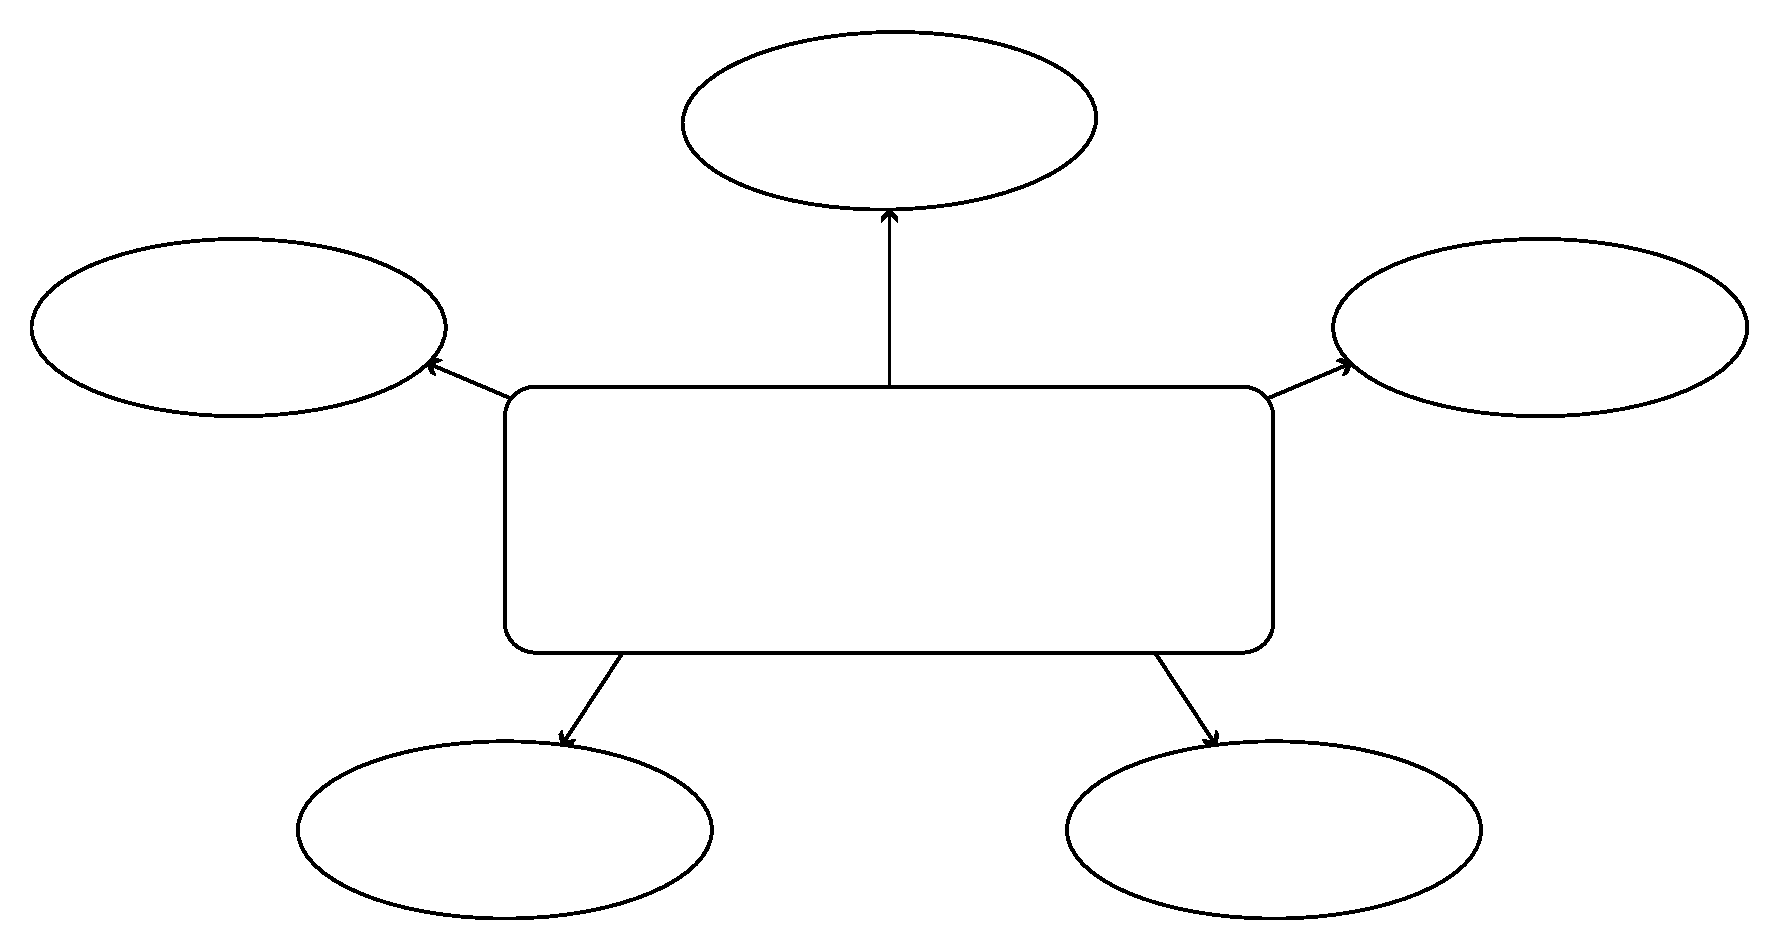
\includegraphics[width=\linewidth]{ch3_theorie_framework/abbildungen/framework.pdf}};
        % Koordinatensystem für die Grafik
        \begin{scope}[x={(image.south east)},y={(image.north west)}]
            % Textpositionen anpassen:
            \node at (0.5,0.45) {\LARGE\parbox{8cm}{\centering\textbf{Framework\\Anomaliedetektion}}};
            \node at (0.13,0.65) {\large \hyperref[subsec:evaluation]{Evaluation}};
            \node at (0.87,0.65) {\large \parbox{3cm}{\centering\hyperref[sec:technologische_grundlagen]{Technologische\\Grundlagen}}};
            \node at (0.5,0.87) {\large\hyperref[ch:zielsetzung]{Zielsetzung}};
            \node at (0.28,0.13) {\large \parbox{3cm}{\centering\hyperref[sec:datenverarbeitung]{Daten-\\verarbeitung}}};
            \node at (0.72,0.13) {\large \parbox{3cm}{\centering\hyperref[sec:zustandsueberwachung]{Zustands-\\überwachung}}};
        \end{scope}
    \end{tikzpicture}
    \caption{Framework der Entwicklung eines Systems zur Anomaliedetektion}
~\label{fig:pdm_framework}
\end{figure}

\subsection{Technologische Grundlagen}\label{sec:technologische_grundlagen}
Die technologischen Grundlagen dieser Arbeit stützen sich auf die in der \ac{sspx1} verbauten Sensoren, die präzise Systemdaten erfassen
und kontinuierlich überwachen. Zu den erfassten Parametern gehören unter anderem die Temperatur und Auslastung von \ac{gpu} und \ac{cpu},
die Auslastung des Arbeitsspeichers sowie die Strom- und Leistungsaufnahme des Blitzmoduls.

Ein zentraler Baustein ist die Nutzung moderner \ac{iot}-Technologien in Kombination mit dem industriellen Kommunikationsstandard \ac{opcua}.\
Dieser Standard basiert auf Ethernet TCP/IP und ermöglicht einen effizienten und sicheren Zugriff auf die Sensordaten der \ac{sspx1} und
deren Übertragung an eine Anwenderschnittstelle nach dem Client-Server-Prinzip~\cite[S.~470]{Babel2024}.

Da die Sensoren teilweise von unterschiedlichen Herstellern stammen und Messdaten in verschiedenen Formaten bereitstellen, sorgt \ac{opcua}
für eine einheitliche und standardisierte Kommunikation. Die Daten werden dabei im kompakten \textit{\ac{opcua} Binary}-Format~\cite{iec62541}
erfasst, wodurch eine performante und ressourcenschonende Datenübertragung ermöglicht wird. Anschließend werden die Daten an den \ac{opcua}-Server
übermittelt und in der zugrundeliegenden \ac{sql}-Datenbank gespeichert. 

Durch diese Architektur wird eine herstellerübergreifende Interoperabilität gewährleistet, weshalb \ac{opcua} besonders für den betrachteten
Anwendungsfall geeignet ist. Die hohe Skalierbarkeit und Erweiterbarkeit des Standards ermöglicht zudem die einfache Integration
weiterer Sensoren und Systeme, wodurch zukünftige Erweiterungen ohne grundlegende Anpassungen der bestehenden Infrastruktur möglich
sind. Diese sog.~\textit{Cyber Physical Systems} ermöglichen also die Verbindung von mechanischen Komponenten über Netzwerke und sind
essentiell für die Architektur dieser Arbeit.

Ein weiterer Vorteil der Nutzung von \ac{opcua} liegt in der serviceorientierten Architektur, die eine flexible Kommunikation
zwischen Client und Server ermöglicht. Der Client fungiert hierbei als Kommunikationsbrücke, die Anfragen und Antworten zwischen
der Anwenderschnittstelle und dem Server verwaltet. Die \ac{opcua}-Kommunikations-Stacks unterstützen dabei die Datenverarbeitung und
gewährleisten eine robuste Übertragung, indem sie eng mit dem Speicher- und Dateisystem des Servers zusammenarbeiten. Zu den
wesentlichen Ereignissen der Client-Server-Kommunikation gehören~\cite{Babel2024}~\cite{iec62541}~\cite{Mao2024}:
\begin{itemize}
    \item \textbf{Message Requests:} Anfragen des Clients zur Datenabfrage oder -übertragung
    \item \textbf{Message Responses:} Antworten des Servers auf die Anfragen des Clients
    \item \textbf{Order Requests:} Aufrufe zur Ausführung bestimmter Serveraktionen
    \item \textbf{Notifications:} Benachrichtigungen über Änderungen oder Ereignisse im System
\end{itemize}

Darüber hinaus kann der \ac{opcua}-Server als Bindeglied zwischen mehreren physischen Geräten oder auch als Cloud-Service fungieren,
was die Skalierbarkeit weiter erhöht und die Nutzung in verteilten Systemen erlaubt. Im Rahmen dieser Arbeit wird auf diese Funktionalität
jedoch verzichtet, da jede \ac{sspx1} einen eigenen Server betreibt, der sämtliche aufgenommene Messdaten bereitstellt.

\subsection{Zustandsüberwachung}\label{sec:zustandsueberwachung}
Ein wesentlicher Grund für ineffiziente Wartungsmaßnahmen liegt im unzureichenden Zugang zu Daten, die frühe Hinweise auf
potenzielle Schäden oder Ausfälle liefern könnten~\cite[S.~2]{Mobley2002}. Predictive Maintenance basiert auf der Voraussetzung, dass
Daten über den Zustand des betreffenden Systems oder der betreffenden Komponente zuverlässig verfügbar sind. Die Bereitstellung der
Daten erfolgt wie oben beschrieben mithilfe von \ac{opcua} und die Zustandsüberwachung sensorbasiert.

Zu Beginn der Arbeit und in der Entwicklungsphase wird die Zustandsüberwachung einen inspektionsbasierten Ansatz verfolgen. Das
bedeutet, dass nach willkürlichen oder festelegten Intervallen immer auf die vom \ac{opcua} Server zur Verfügung gestellten Daten
zugegriffen wird und diese Datensätze dann analysiert und weiterverarbeitet werden. Die Wahl dieser Methode basiert auf der
geringeren Komplexität der Implementierung in frühen Entwicklungsphasen und hat zur Folge, dass ein konsistenter Datensatz einen
besseren Vergleich und Feinabstimmung von Parametern der Analysetools ermöglicht.

Online Predictive Maintenance erweitert diesen Ansatz, indem sie eine Überwachung des Systemzustands in Echtzeit im laufenden Betrieb
ermöglicht. Dabei werden Daten oder andere relevante Parameter in regelmäßigen Abständen automatisch erfasst. Nicht alle erfassten
Daten werden analysiert; vielmehr wird gezielt ausgewählt, welche Informationen für die Analyse und die Ableitung von Wartungsmaßnahmen
notwendig sind~\cite{Lindstroem2017}. 
% hier könnte man zu einem späteren zeitpunkt schreiben, wie genau die zustandsüberwachung durchgeführt wurde

Die aufgenommenen Messdaten zur Zustandsüberwachung liegen als multivariate Zeitserie vor. Das bedeutet, dass alle aufgenommenen Messwerte
mit einem Zeitstempel versehen sind. Dabei besteht die Möglichkeit, die Intervalle für die Messdatenaufnahme unterschiedlich einzustellen.
Ein Temperaturwert unterliegt langsameren Schwankungen und kann daher in größeren Intervallen aufgenommen werden, als beispielsweise die
Strom- oder Leistungsaufnahme des Blitzmoduls, wo auch kurzzeitige Spitzen und Ausreißer zuverlässig erkannt werden müssen.
% Für den Moment sind jedoch alle Messintervalle gleich. auch hier: später ggf. überarbeiten

\subsection{Datenverarbeitung}\label{sec:datenverarbeitung}
Durch die kontinuierliche Aggregation von Messdaten der \ac{sspx1} entstehen sehr große, hochdimensionale Datensätze. Jeder Datenpunkt in
der Zeitserie $S$ ist mehrdimensional. Eine Zeitserie ist eine Menge der Mächtigkeit $n$. Alle $n$ Elemente sind reellwertige
$d$~-~dimensionale Datenpunkte $S_i\,\in\,\mathbb{R}^{d}$~\cite{Schmidl2022}. Ebenfalls lässt sich eine Zeitserie $S$ der Länge $n$ und
Dimensionalität $d$ als Matrix wie in \hyperref[eq:timeseries_matrix_sum]{Gl. \Ref*{eq:timeseries_matrix_sum}a} definieren. $x_{i}^{j}$ ist
der $i$-te Skalar der $j$-ten Dimension einer Serie $S$. Für die Dimension $j={0,\dots,d}$ der Zeitserie $S$ entspricht jede Dimension
einem Messwert im Datensatz. Da es sich um eine Zeitserie handelt, entsprechen die Indizes $i={0, \dots, n}$ den Zeitstempeln der
aufgenommenen Messwerte~\cite{Wenig2024}. Desweiteren wird eine \textit{univariate} Zeitserie als eine eindimensionale Menge definiert,
während eine \textit{multivariate} Zeitserie mehrdimensionale Werte beinhaltet. Im Kontext der Arbeit sind vorrangig multivariate
Zeitserien relevant.

\begin{equation}
    S=\{\,S_1,\,S_2,\,\dots\,,\,S_n\,\}\label{eq:timeseries_set}
\end{equation}

\begin{equation}
    \setcounter{equation}{1}
        \begin{subequations}
        \setlength{\arraycolsep}{1em}
        \renewcommand{\arraystretch}{1.5}
        \begin{aligned}
            S &=
            \begin{bmatrix} 
                x_{0}^{0} & \cdots & x_{0}^{d} \\
                \vdots & \ddots & \vdots \\
                x_{n}^{0} & \cdots & x_{n}^{d} 
            \end{bmatrix} 
            && \text{(a)} \\[1.5em]
            S &= \sum_{i=0}^{n}\,\sum_{j=0}^{d}\,x_{i}^{j} \cdot E_{ij}
            && \text{(b)}\\[1.5em]
            E_{32} &=
            \begin{bmatrix}
                0 & 0 & 0 & 0 \\
                0 & 0 & 0 & 0 \\
                0 & 1 & 0 & 0 \\
                0 & 0 & 0 & 0 \\
            \end{bmatrix}
            && \text{(c)} \\[1.5em]
        \end{aligned}
    \end{subequations}
\label{eq:timeseries_matrix_sum}
\end{equation}

Alternativ kann die Zeitserie $S$ gem.~\hyperref[eq:timeseries_matrix_sum]{Gl. \Ref*{eq:timeseries_matrix_sum}b} auch als Linearkombination
von Standardmatrizen geschrieben werden~\cite[S.~8]{Voigt2012}. Die elementweise Darstellung beschreibt die Matrix $S$ als Summe von
gewichteten Standardmatrizen $E_{ij}$, wobei jede Standardmatrix $E_{ij}$ genau an der Position $(i,j)$ den Wert 1 hat und sonst 0 ist.
\hyperref[eq:timeseries_matrix_sum]{Gl.~\Ref*{eq:timeseries_matrix_sum}c} verdeutlicht dies beispielhaft an der 4$\times$4 Einheitsmatrix
$E_{32}$.

\begin{figure}[t!]
    \centering
    \begin{tikzpicture}
        \node[anchor=south west,inner sep=0] (image) at (0,0) {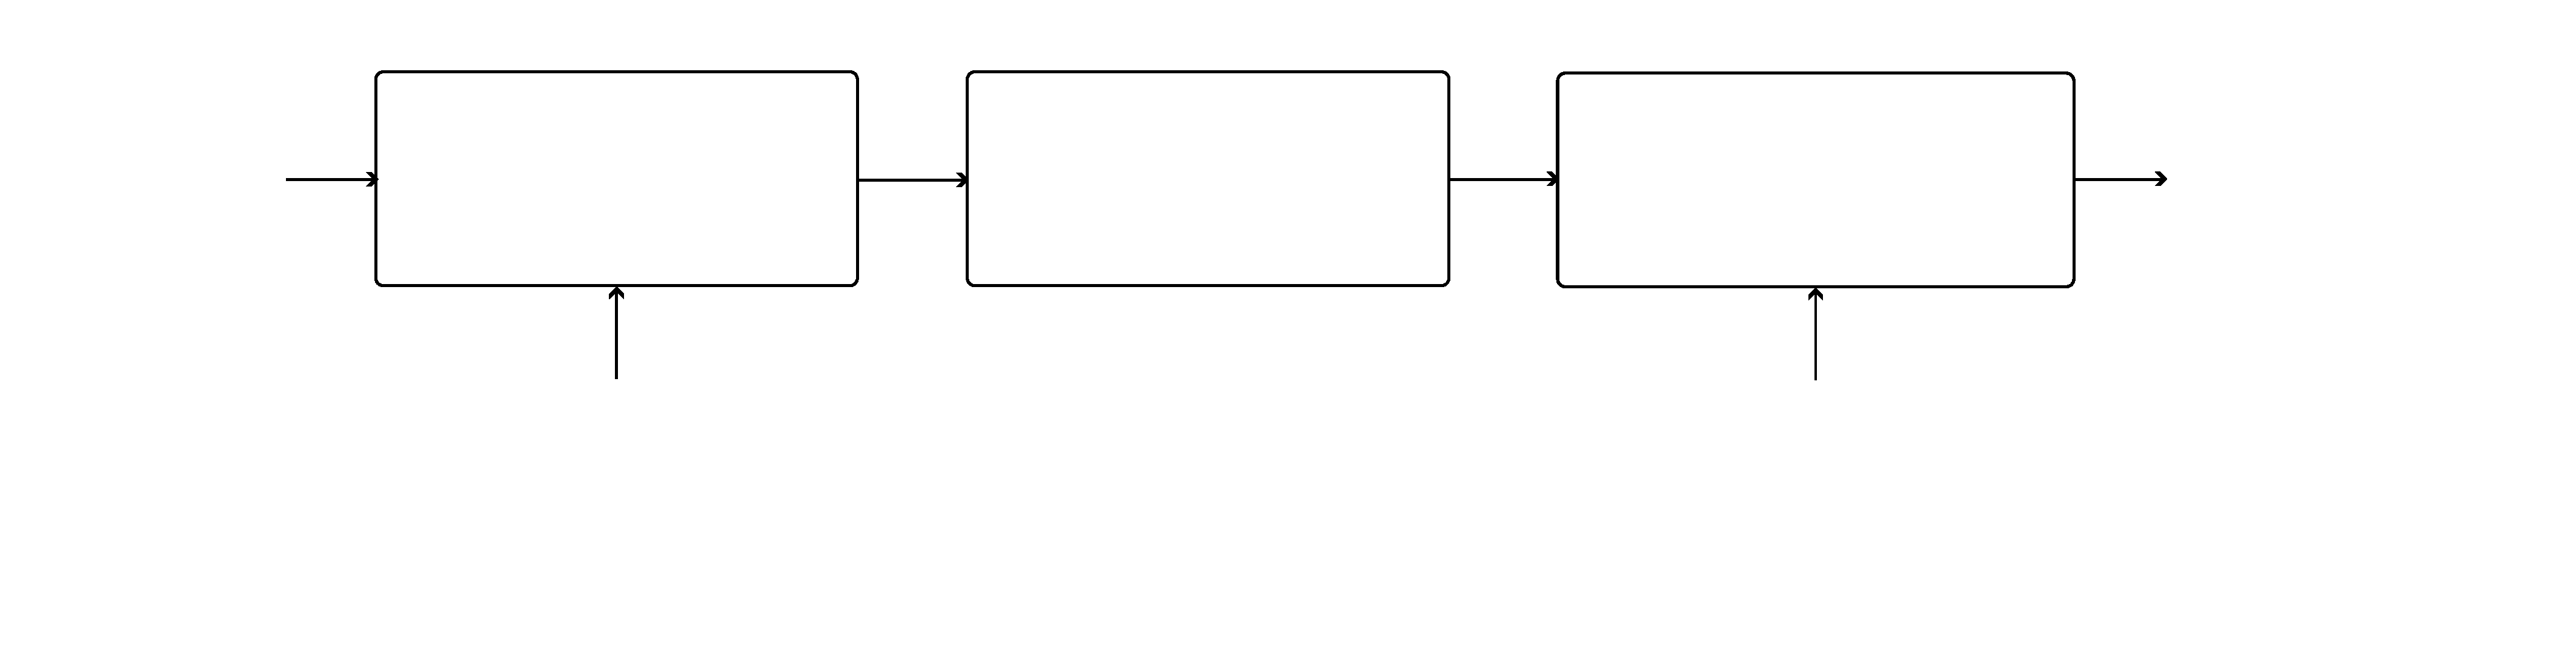
\includegraphics[width=1\linewidth]{ch3_theorie_framework/abbildungen/data_mining.pdf}};
        % Koordinatensystem für die Grafik
        \begin{scope}[x={(image.south east)},y={(image.north west)}]
            % Textpositionen anpassen:
            \node at (0.059,0.725) {\large\centering Rohdaten};
            \node at (0.2365,0.725) {\large \parbox{6cm}{\centering Vorverarbeitung\\der Daten}};
            \node at (0.47,0.725) {\large Data Mining};
            \node at (0.705,0.725) {\large \parbox{6cm}{\centering Nachverarbeitung\\der Daten}};
            \node at (0.904,0.725) {\large \parbox{3cm}{\centering Information}};
            \node at (0.2365,0.2) {\large \parbox{6cm}{\centering Dimensionalität reduzieren\\Normierung\\Subsets bilden}};
            \node at (0.705,0.2) {\large \parbox{6cm}{\centering Visualisierung\\Anomaliedetektion\\Anomalien bewerten}};
        \end{scope}
    \end{tikzpicture}
    \caption{\centering Typischer Data Mining Workflow vom Eingang der Quelldaten bis zum Informationsgewinn}
~\label{fig:data_mining}
\end{figure}

\textit{Data Mining} spielt in dem Zusammenhang eine große Rolle. Unter Data Mining versteht man das Finden relevanter Informationen,
Muster oder Trends in großen Datensätzen. Mithilfe verschiedener Data Mining Techniken können so Voraussagen über künftige Ereignisse oder
Beobachtungen getroffen werden. Der Prozess des Data Minings lässt sich anhand von~\hyperref[fig:data_mining]{Abb.~\Ref*{fig:data_mining}}
visualisieren. Dabei gehen zunächst Rohdaten aus den zahlreichen Sensoren hervor und liegen bedingt durch das \ac{sql}-Format in einer
relationalen Datenbank vor. Der nächste Schritt der Vorverarbeitung erfolgt dann, damit die Daten in einem handlichen und analysierbaren
Format vorliegen. Daher werden diese sowohl in ihrer Dimensionalität reduziert als auch normiert. Gegebenenfalls werden auch
kontextbezogene Subsets gebildet, z.~B.~für Tageszeiten oder sonstige Bedingungen~\Cite[Kap.~1]{Tan2014}.

Zur Datenverarbeitung gehören auch spezifische Herausforderungen, die die Entwicklung neuer Data Mining Techniken vorangetrieben haben.
Dazu gehört unter anderem die Skalierbarkeit eines Algorithmus, um zu gewährleisten, dass auch sehr große und immer größer werdende
Datensätze mit der gleichen Präzision und Qualität verarbeitet werden. Desweiteren zählen auch die Hochdimensionalität und Heterogenität
der vorliegenden Datensätze zu großen Herausforderungen bei der Findung geeigneter Algorithmen. Für hochdimensionale Daten muss im Voraus
im Rahmen der Vorverarbeitung eine Reduzierung der Dimensionalität stattfinden, d.h.~irrelevante oder redundante Datenpunkte werden
entfernt oder mit ähnlichen Datenpunkten zusammengefasst. Auch statistische Abhängigkeiten und Unabhängigkeiten sowie Korrelationen
werden in diesem Schritt mit berücksichtigt. Die Heterogenität eines Datensatzes zeigt sich beispielsweise durch das Auftreten von
Datenpunkten mit unterschiedlichen physikalischen Einheiten, wie Temperaturwerte und solche zur Festplattenauslastung und
-schreibgeschwindigkeit. Bevor ein Datensatz also einem Algorithmus zur Anomaliedetektion übergeben werden kann, muss eine adäquate
Vorverarbeitung stattfinden, denn nur so können auch relevante Ergebnisse erzeugt werden.

% weitere inhalte dieses abs.: wie wird die dimensionalität zb verringert? pca oder ähnliche verfahren. abhängig von den gewählten
% algorithmen, die getestet werden sollen

\subsection{Evaluation}\label{subsec:evaluation}
% hier soll kurz vorgestellt werden, anhand welcher kriterien und mit welchen verfahren ein algorithmus bewertet werden soll
% zb. rechendauer, anomaliequote etc.
Zur Vergleichbarkeit und Gegenüberstellung der gewählten Algorithmen aus~\hyperref[sec:algorithmen]{Abs.~\Ref*{sec:algorithmen}} werden
entsprechend der Detektionsklasse unterschiedliche Evaluierungsmethoden verwandt.

Grundsätzlich ist es von höchster Bedeutung, dass für gleiche Detektionsklassen gleiche Evaluierungsmethoden angewandt werden, um einen
aussagekräftigen Vergleich zu gewährleisten. Dabei ist eine der gängigsten Methoden zur Evaluierung von Klassifizierungsalgorithmen
jeglicher Art der F$\beta$-Score, der das harmonische Mittel zwischen den von Lewis in~\cite{Lewis1991} benannten Größen \textit{Precision}
und \textit{Recall} bildet. Precision und Recall ergeben sich aus einem Verhältnis der Größen \textit{True Positive}, \textit{False
Positive} und \textit{False Negative}. Der Parameter $\beta$ ist ein Gewichtungsfaktor für das Verhältnis von Precision und Recall.

\setlength{\jot}{15pt}
\begin{align}
    \text{Precision} &= \frac{\text{TP}}{\text{TP} + \text{FP}} \label{eq:precision} \\
    \text{Recall} &= \frac{\text{TP}}{\text{TP} + \text{FN}} \label{eq:recall} \\
    F_{\beta} &= (1\,+\,\beta^2) \cdot \frac{\text{Precision} \cdot \text{Recall}}{\beta^2\,\cdot\,\text{Precision} + \text{Recall}}
    \label{eq:fbeta}
\end{align}

\begin{figure}[b!]
    \centering
        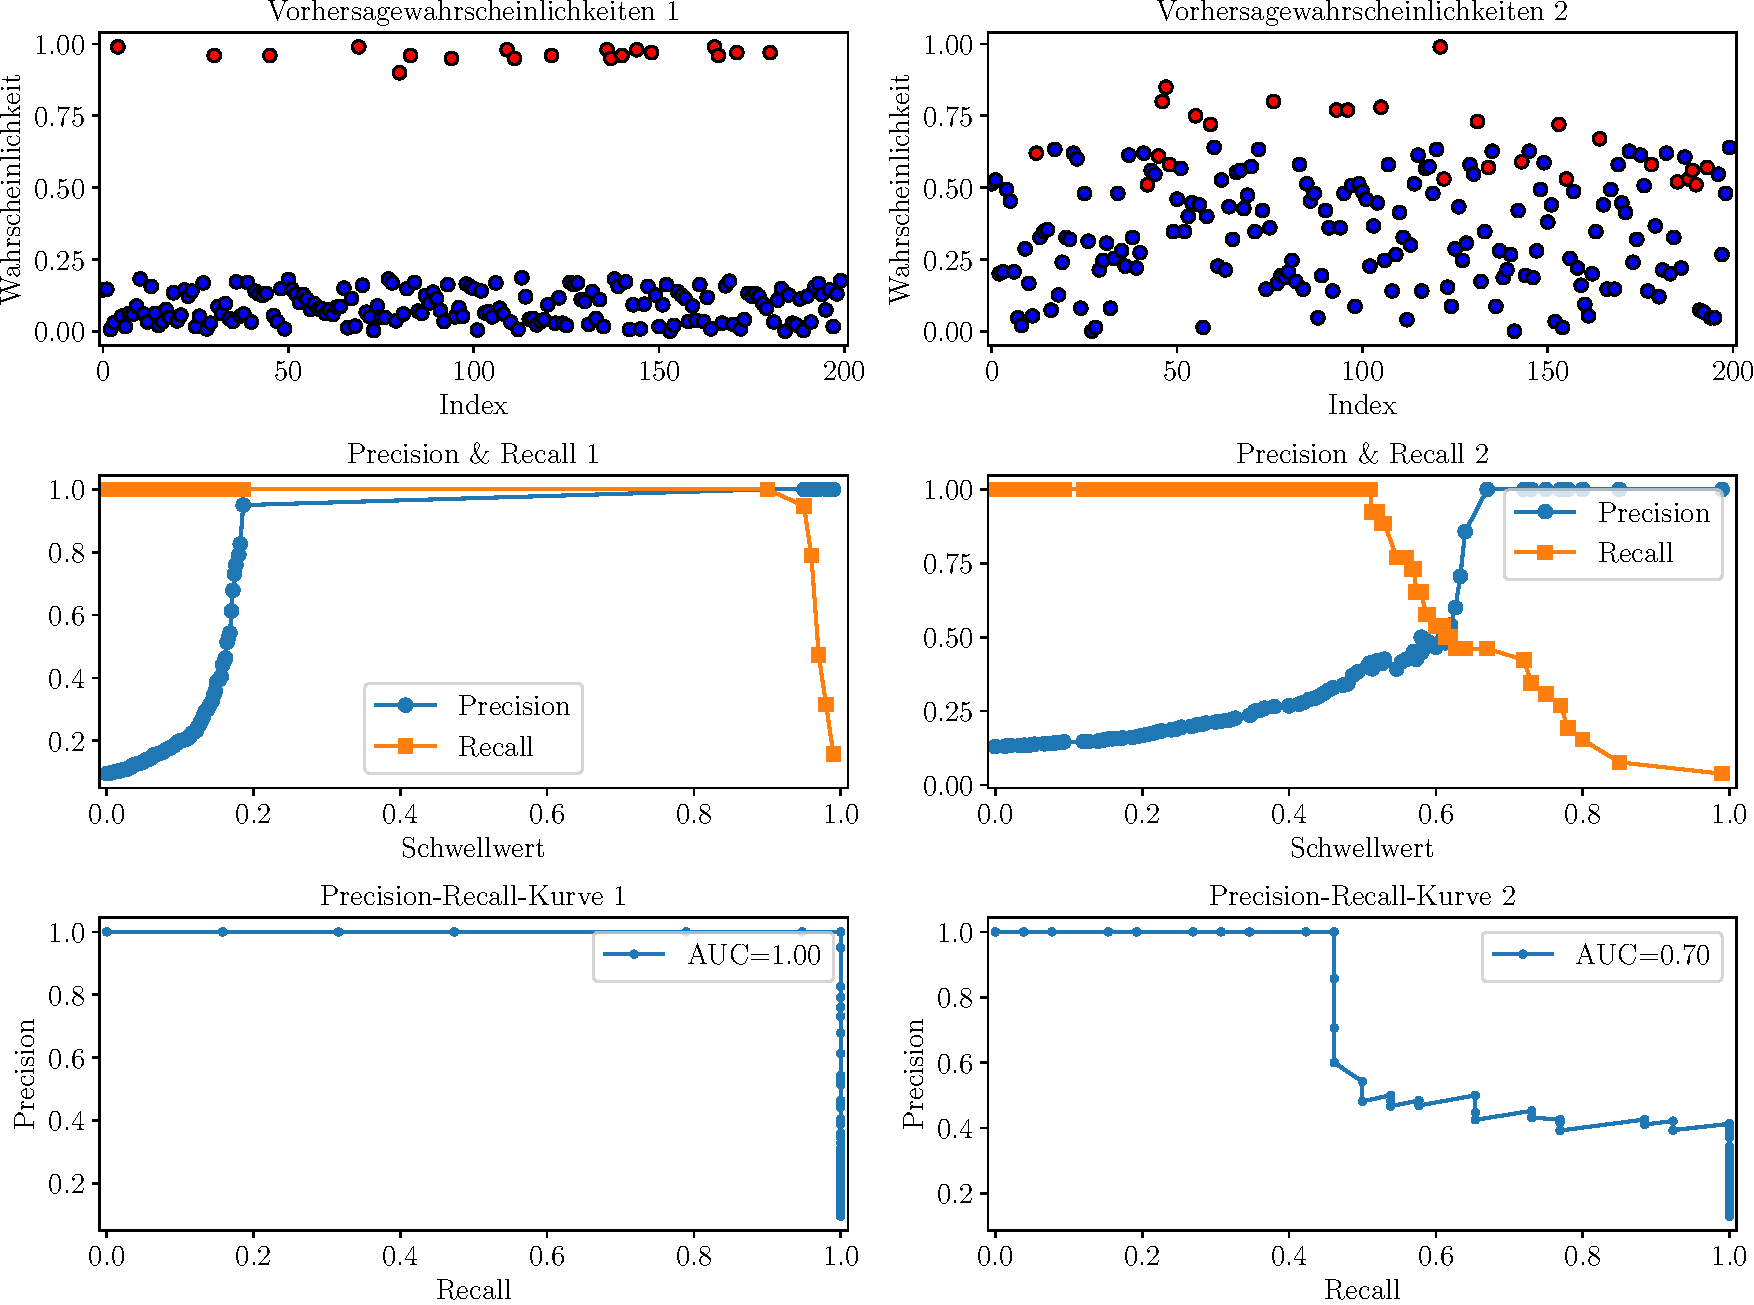
\includegraphics[width=1\linewidth]{ch3_theorie_framework/abbildungen/pr-kurve.pdf}
    \caption{\centering Zwei Beispielszenarien als Resultat der Anomaliedetektion eines Datensatzes. In der ersten Reihe sind die resultierenden
    Vorhersagewahrscheinlichkeiten aufgetragen, mit den roten Punkten als tatsächliche Anomalien. Die Anomalien in Datensatz 1 sind im Vergleich
    zu Datensatz 2 deutlich präziser vorhergesagt, was die \ac{prkurve} auch widerspiegelt.}
~\label{fig:auc_pr_beispiel}
\end{figure}

Um die optimale Entscheidungsschwelle zu finden und auch einen Überblick über die Performance eines Algorithmus über mehrere Schwellwerte
zu erhalten, eignet sich die \ac{prkurve}, die in~\hyperref[fig:auc_pr_beispiel]{Abb.~\Ref*{fig:auc_pr_beispiel}} dargestellt
ist. Aus der \ac{prkurve} kann dann die sogenannte \ac{aucpr}
berechnet werden, die als Indikator dafür dient, wie gut ein Modell über alle möglichen Schwellwerte hinweg zwischen der positiven und
negativen Klasse~-~im Bezug auf Aomalieerkennung entspricht das normal und anomal~-~unterscheidet, wobei sie insbesondere bei
unausgewogenen Datensätzen aussagekräftig ist~\cite{Davis2006}~\cite{Schmidl2022}. Unter unausgewogenen Daten versteht man in diesem Zusammenhang,
dass die große Mehrheit der Datenpunkte normal ist, während lediglich vereinzelte Punkte eine Anomalie darstellen.

Mithilfe der \ac{prkurve} kann der Schwellwert ermittelt werden, der den optimalen F$\beta$-Score zurückgibt. Dieser ist allerdings
alleine nicht aussagekräftig genug, da bei echten Daten nie gegeben sein kann, dass diese optimale Schwelle aufgrund der Unsicherheit der
Daten gefunden wird. Dementsprechend ist \ac{aucpr} eine bessere Metrik zur Gegenüberstellung zweier Algorithmen~\cite{Japkowicz2002}.

Aus einem Algorithmus zur Anomaliedetektion geht eine Anomaliebewertung hervor, diese kann als relative Wahrscheinlichkeit interpretiert werden,
mit der ein Algorithmus einen Punkt als Anomalie vorhersagt. Die Einordnung in die Klassen Normal und Anomalie erfolgt anhand eines festzulegenden
Schwellwerts. Für reale Daten liegt die optimale Schwelle zur präzisesten Vorhersage allerdings nicht vor. Die \ac{prkurve} ist demnach auch ein
Maß dafür, wie deutlich ein Algorithmus zwischen normalen und anomalen Punkten unterscheiden kann und wie abhängig seine Performance von der
Wahl der optimalen Schwelle ist~\cite{Japkowicz2002}.

Die linke Spalte in~\hyperref[fig:auc_pr_beispiel]{Abb.~\Ref*{fig:auc_pr_beispiel}} zeigt dies für einen Algorithmus, der die vorliegenden Daten
eindeutig zuordnen kann, da alle detektierten Anomalien eine Wahrscheinlichkeit von über 90 \% aufweisen können, während als normal detektierten
Punkte unter 25 \% liegen. Für einen Schwellwert zwischen diesen beiden Grenzen hat das also immer eine optimale Performance zur Folge. Liegt der
Schwellwert darunter, so wirkt sich das negativ auf die Precision aus, denn so erkennt der Algorithmus dann viele Punkte als False Positives.
Im Gegenzug hat eine zu hohe Schwelle viele False Negatives zur Folge und der Recall Wert sinkt.

Der zweite Algorithmus aus der rechten Spalte in~\hyperref[fig:auc_pr_beispiel]{Abb.~\Ref*{fig:auc_pr_beispiel}} verdeutlicht die Folgen einer
ungenaueren Zuordnung, da normale Punkte mit einer hohen Wahrscheinlichkeit als anomal eingeordnet werden, während wahre Anomalien eine niedrige
Wahrscheinlichkeit erhalten. Das bedeutet, dass sich bei einer Veränderung der Schwelle sowohl Precision als auch Recall verändern, und zeigt
eine stärkere Abhängigkeit des Algorithmus von der Wahl des richtigen Schwellwerts.

Das Beispiel zeigt, dass eine starke Differenzierung zwischen normalen und anomalen Punkten für eine robuste Anomalieerkennung eines Algorithmus
spricht und sich in einem hohen \ac{aucpr} widerspiegeln. Im Umkehrschluss deutet ein niedrigerer \ac{aucpr} Wert darauf hin, dass ein Algorithmus zwar
Anomalien erkennen kann, jedoch nur bei einer optimalen Parametrisierung. Im Allgemeinen ist ein Algorithmus mit hohem \ac{aucpr} zu bevorzugen.